\scanpage{46}
\mspage{\handwritten{14}}
\uline{11.6.}- Let $G$ be a flat $S$-group quasi-compact and quasi-separated over $S$\handwritten{,} such that $\handwritten{\unsure{\mathcal{A}|a}}(G)$ is a flat $\handwritten{\mathcal{O}}_S$-Module $\handwritten{\mathcal{A}}$, and $\handwritten{\mathcal{E}}$ a quasi-coherent and flat $\handwritten{\mathcal{O}}_S$-Module. \deleted{We shall say that}\inserted{\handwritten{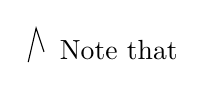
\begin{tikzpicture}[x=1cm,y=1cm,baseline=(n.base)]\node (n) at (0,0) {Note that};\draw (-1.15,-.15)--(-1.05,.28)--(-.95,-.02);\end{tikzpicture}}} a morphism of $S$-functors from $G$ to $\inserted{\handwritten{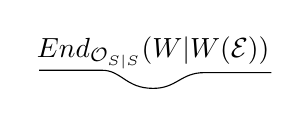
\begin{tikzpicture}[x=1cm,y=1cm,baseline=(n.base)]\node (n) at (0,0) {$\operatorname{End}_{\mathcal{O}_{\unsure{\mathbb{S}|S}}}(\unsure{\mathbb{W}|W}(\mathcal{E}))$};\draw (-1.45,-.22)--(-.65,-.22) .. controls (-.4,-.22) and (-.35,-.45) .. (0,-.45) .. controls (.3,-.45) and (.35,-.25) .. (.65,-.25)--(1.5,-.25);\end{tikzpicture}}}\deleted{\handwritten{\unsure{=|\simeq}\mathcal{H}om_{\mathcal{O}_S}(\mathcal{E},\mathcal{E})}}\handwritten{\simeq\mathcal{H}om}_{\handwritten{\mathcal{O}}_S}(\handwritten{\mathbb{V}}(\handwritten{\mathcal{E}}),\handwritten{\mathbb{V}}(\handwritten{\mathcal{E}}))$ defines an \uline{ac}-\linebreak\uline{tion} of $G$ on $\handwritten{\mathcal{E}}$\handwritten{,} if \inserted{\handwritten{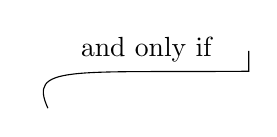
\begin{tikzpicture}[x=1cm,y=1cm,baseline=(n.base)]\node (n) at (0,0) {and only if};\draw (-1.25,-.75) .. controls (-1.5,-.2) and (-1,-.3) .. (1.3,-.28)--(1.3,-.02);\end{tikzpicture}}} the corresponding morphism $\handwritten{\theta}:G\handwritten{\times}_S\handwritten{\mathbb{V}}(\handwritten{\mathcal{E}})\handwritten{\longrightarrow\mathbb{V}}(\handwritten{\mathcal{E}})$ satisfies the following two conditions:

$1^\circ)$ if $\handwritten{\mu}:G\handwritten{\times}_S G\handwritten{\longrightarrow}G$ denotes the structure morphism, the diagram
\diagram{\begin{tikzcd}[ampersand replacement=\&]
G\handwritten{\times}_S G\handwritten{\times}_S\handwritten{\mathbb{V}}(\handwritten{\mathcal{E}})
 \arrow[r,"\operatorname{id}_G\handwritten{\times\theta}"]\arrow[d,"\handwritten{\mu\times}\operatorname{id}_{\handwritten{\mathbb{V}(\mathcal{E})}}"']
\& G\handwritten{\times}_S\handwritten{\mathbb{V}}(\handwritten{\mathcal{E}})\arrow[d,"\handwritten{\theta}"]\\
G\handwritten{\times}_S\deleted{X}\handwritten{\mathbb{V}}(\handwritten{\mathcal{E}})\arrow[r,"\handwritten{\theta}"]
\& \handwritten{\mathbb{V}}(\handwritten{\mathcal{E}})
\end{tikzcd}}
\inserted{\figure{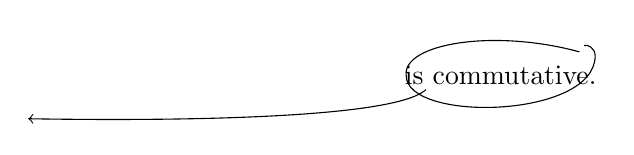
\begin{tikzpicture}[x=1cm,y=1cm]\handwritten{\draw (1,.3) .. controls (-.1,.6) and (-1.25,.4) .. (-1.2,0) .. controls (-1.2,-.6) and (1.2,-.55) .. (1.2,.25) .. controls (1.2,.35) and (1.1,.4) .. (1.06,.38);\draw[->] (-.95,-.18) .. controls (-1.45,-.65) and (-5.8,-.55) .. (-6,-.55);}\node at (0,0) {is commutative.};\end{tikzpicture}}}

$2^\circ)$ if $\handwritten{\varepsilon}:S\handwritten{\to}G$ is the unit section of $G$, the diagram
\diagram{\begin{tikzcd}[ampersand replacement=\&]
S\handwritten{\times}_S\handwritten{\mathbb{V}}(\handwritten{\mathcal{E}})
 \arrow[rr,"\handwritten{\varepsilon\times}\operatorname{id}_{\handwritten{\mathbb{V}(\mathcal{E})}}"]
\& \& G\handwritten{\times}_S\handwritten{\mathbb{V}}(\handwritten{\mathcal{E}})\arrow[dl,"\handwritten{\theta}"]\\
\& \handwritten{\mathbb{V}}(\handwritten{\mathcal{E}})\arrow[ul,"\handwritten{\sim}"'] \&
\end{tikzcd}}
\inserted{\figure{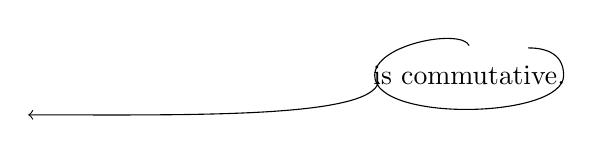
\begin{tikzpicture}[x=1cm,y=1cm]\handwritten{\draw (0,.38) .. controls (-.1,.6) and (-1.2,.4) .. (-1.2,0) .. controls (-1.2,-.6) and (1.2,-.55) .. (1.2,0) .. controls (1.2,.32) and (.9,.35) .. (.75,.35);\draw[->] (-1.15,-.08) .. controls (-1.25,-.55) and (-3.6,-.5) .. (-5.6,-.5);}\node at (0,0) {is commutative.};\end{tikzpicture}}}

It amounts\inserted{\handwritten{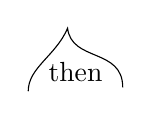
\begin{tikzpicture}[x=1cm,y=1cm,baseline=(n.base)]\node (n) at (0,0) {then};\draw (-.6,-.25) .. controls (-.6,.05) and (-.25,.2) .. (-.1,.55) .. controls (-.05,.12) and (.6,.3) .. (.6,-.2);\end{tikzpicture}}} to the same thing to say that the morphism $\handwritten{\rho}:\inserted{\handwritten{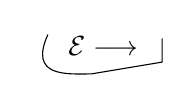
\begin{tikzpicture}[x=1cm,y=1cm,baseline=(n.base)]\node (n) at (0,0) {$\mathcal{E}\longrightarrow$};\draw (-.7,.15) .. controls (-.95,-.4) and (-.45,-.35) .. (-.15,-.35)--(.75,-.2)--(.75,.1);\end{tikzpicture}\begin{tikzpicture}[x=1cm,y=1cm]\draw (0,0)--(0,-.38);\end{tikzpicture}}}\handwritten{\mathcal{A}}(G)\handwritten{\otimes}_{\handwritten{\mathcal{O}}_{\unsure{\mathbb{S}|S}}}\handwritten{\mathcal{E}}$ deduced from $\handwritten{\theta}$ satisfies the following two axioms:
\margin{\handwritten{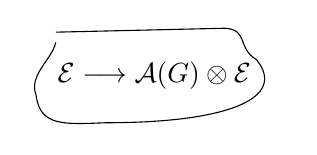
\begin{tikzpicture}
\draw (-1.25,.55)--(.9,.6) .. controls (1.2,.58) and (1.05,.35) .. (1.3,.2) .. controls (1.7,-.3) and (.9,-.6) .. (-.6,-.6) .. controls (-1.15,-.62) and (-1.45,-.65) .. (-1.5,-.25) .. controls (-1.6,0) and (-1.3,.2) .. (-1.25,.42);
\node at (0,0) {$\mathcal{E}\longrightarrow\mathcal{A}(G)\otimes\mathcal{E}$};
\end{tikzpicture}}}

(CM1) If $\handwritten{\Delta}:\handwritten{\mathcal{A}\longrightarrow\mathcal{A}\otimes\mathcal{A}}=\handwritten{\mathcal{A}}(G\handwritten{\times}_S G)$ is the homomorphism $\handwritten{\mathcal{A}(\theta)}$, the diagram
\diagram{\handwritten{\begin{tikzcd}[ampersand replacement=\&]
\mathcal{A}\otimes\mathcal{A}\otimes\mathcal{A}
\& \mathcal{A}\otimes\mathcal{E}\arrow[l,"\operatorname{id}_{\mathcal{A}}\otimes\rho"']\\
\mathcal{A}\otimes\mathcal{E}\arrow[u,"\Delta\otimes\operatorname{id}_{\mathcal{E}}"]
\& \mathcal{A}\arrow[u,"\rho"']\arrow[l,"\rho"']
\end{tikzcd}}}
\inserted{\figure{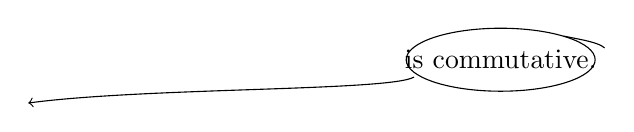
\begin{tikzpicture}[x=1cm,y=1cm]\handwritten{\draw (0,0) ellipse (1.2 and .4);\draw (.8,.3) .. controls (1.05,.25) and (1.24,.22) .. (1.32,.15);\draw[->] (-1.1,-.22) .. controls (-1.4,-.4) and (-4.5,-.35) .. (-6,-.55);}\node at (0,0) {is commutative.};\end{tikzpicture}}}

(CM2) If $\handwritten{\eta}:\handwritten{\mathcal{A}\to\mathcal{O}}_S$ is the homomorphism $\handwritten{\mathcal{A}(\varepsilon)}$, the diagram
\diagram{\handwritten{\begin{tikzcd}[ampersand replacement=\&]
\mathcal{O}_S\otimes\mathcal{E}
\& \& \mathcal{A}\otimes\mathcal{E}\arrow[ll,"\eta\otimes\operatorname{id}_{\mathcal{E}}"']\\
\& \mathcal{E}\arrow[ul,"\sim"']\arrow[ur,"\rho"']\&
\end{tikzcd}}}
\inserted{\figure{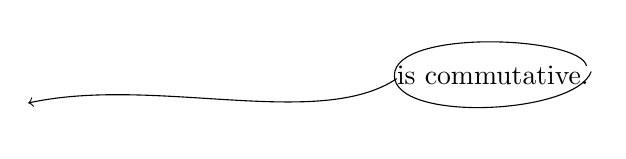
\begin{tikzpicture}[x=1cm,y=1cm]\handwritten{\draw (1.19,.12) .. controls (1.12,.5) and (-1.25,.6) .. (-1.25,0) .. controls (-1.25,-.6) and (1.05,-.5) .. (1.25,.05);\draw[->] (-1.22,-.04) .. controls (-2.2,-.7) and (-4.3,.0) .. (-5.9,-.35);}\node at (0,0) {is commutative.};\end{tikzpicture}}}

It amounts to the same thing to say that the morphism $\handwritten{\theta}_{\mathrm{af}}:G_{\mathrm{af}}\handwritten{\times}_S\handwritten{\mathbb{V}}(\handwritten{\mathcal{E}})\handwritten{\longrightarrow\mathbb{V}}(\handwritten{\mathcal{E}})$ corresponding to $\handwritten{\rho}$ defines an action of $G_{\mathrm{af}}$ on $\handwritten{\mathcal{E}}$ \deleted{\handwritten{\unsure{(compare I)|(Exposé I)}}} \inserted{\handwritten{(compare I 4.2)}}.

Consequently, there is a one-to-one correspondence between actions of $G$ on $\handwritten{\mathcal{E}}$ and ac-\linebreak tions of $G_{\mathrm{af}}$ on $\handwritten{\mathcal{E}}$.

\uline{\handwritten{L}emma} 11.7.- Let $G$ be an $S$-group quasi-compact and quasi-separated over $S$\handwritten{,}\inserted{\handwritten{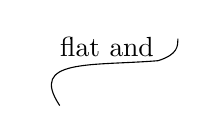
\begin{tikzpicture}[x=1cm,y=1cm,baseline=(n.base)]\node (n) at (0,0) {flat and};\draw (-.6,-.75) .. controls (-1,-.15) and (-.2,-.25) .. (.65,-.18) .. controls (.9,-.1) and (.9,0) .. (.9,.1);\end{tikzpicture}}} such that $\handwritten{\mathcal{A}}(G)$ is
% archive sheet number: 45
